\chapter{Vergleichende Evaluation}
Die realisierten Implementierungen lassen zwei Vergleiche zu: 
\begin{itemize}
\item Node.js-server mit socket.io-Websocket-Server vs. node.js-Server mit HTML5-Websocket-Server, wobei die Javascript-Clients sich nur marginal unterscheiden.
\item Javascript-Client vs. Dart-Client, wobei beide auf denselben node.js-Server mit HTML5-Websocket-Server zugreifen
\end{itemize}

\section{Socket.io-Websocket vs. HTML5-Websocket}
\subsection{Implementierungsaufwand}
Anzahl zeilen code

\subsection{Latenzzeit}
querytime

time received
\begin {figure}[H]
\begin{center}
  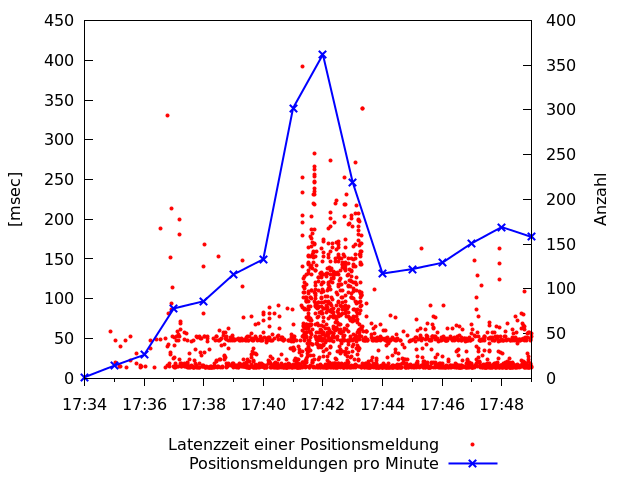
\includegraphics[width=4.5in]{images/latency_timeReceived_socket_io.png}
\end{center}
\caption{socket.io-Websocket-Server: Latenzzeit der Positionsmeldungen und Anzahl empfangener Schiffe}
\end {figure}

\begin {figure}[H]
\begin{center}
  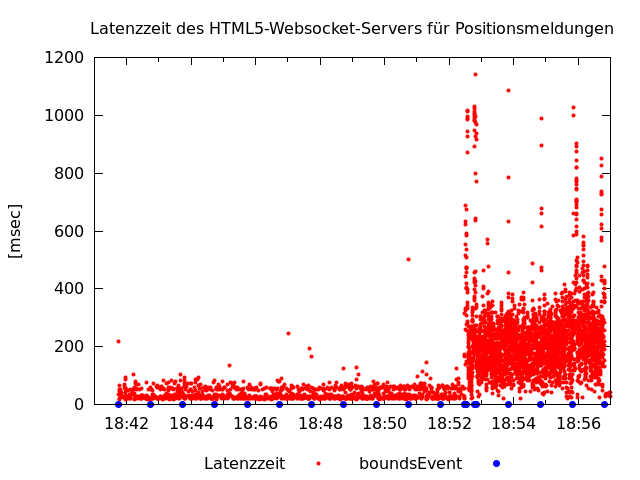
\includegraphics[width=4.5in]{images/latency_timeReceived_HTML5.png}
\end{center}
\caption{HTML5-Websocket-Server: Latenzzeit der Positionsmeldungen und Anzahl empfangener Schiffe}
\end {figure}


\subsection{Performance}
paintToMap

\subsection{Browserunterstützung}
Firefox, Chrome, IE, Safari


\section{Javascript-Client vs. Dart-Client} 
\subsection{Implementierungsaufwand}

\subsubsection{js-Client}
Zeilen Code



\subsection{Latenzzeit}
queryTime

\subsection{Performance}
paintToMap
\newpage

\begin {figure}[H]
\begin{center}
  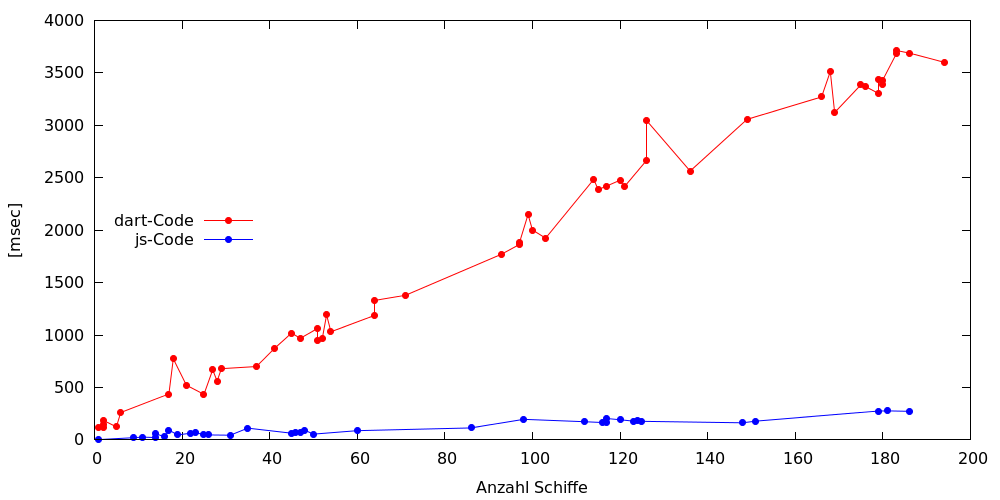
\includegraphics[height=2.3in]{images/Dartium.png}
\end{center}
 \caption{Dauer des Renders in Dartium}
\end {figure}


\begin {figure}[H]
\begin{center}
  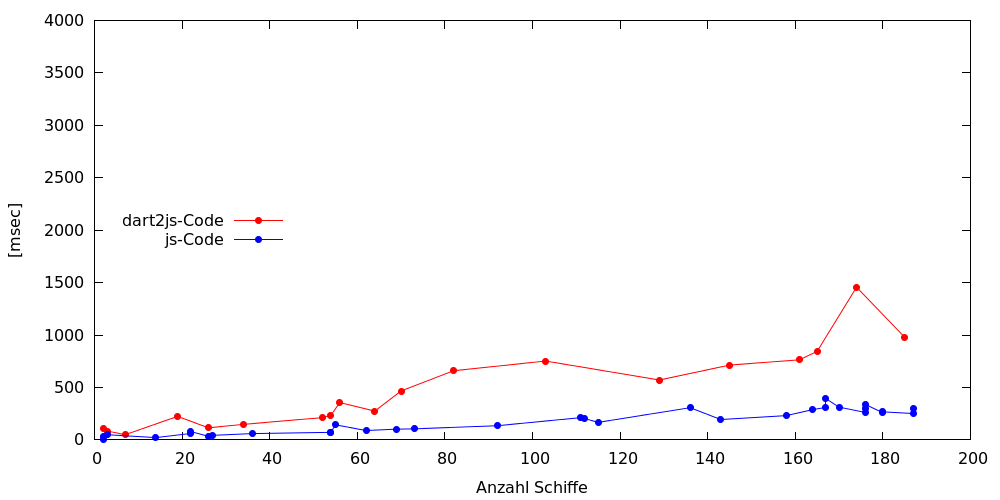
\includegraphics[height=2.3in]{images/Chrome.png}
\end{center}
 \caption{Dauer des Renders in Chrome}
\end {figure}


\begin {figure}[H]
\begin{center}
  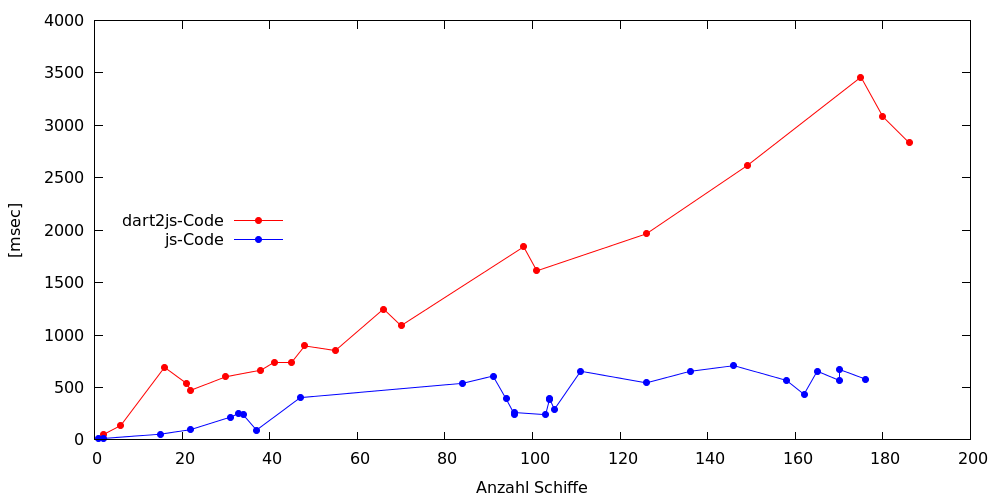
\includegraphics[height=2.3in]{images/Firefox.png}
\end{center}
 \caption{Dauer des Renders in Firefox}
\end {figure}


\subsection{Browserunterstützung}
\subsubsection{Dartium}

\subsubsection{Firefox, Chrome, IE, Safari}

Der dart-Client kompiliert den in Dart geschriebenen Code zu Javascript.

Dabei traten Fehler auf, die unter Dartium (also im originalen Dart-Code) nicht auftraten.
1. Wird innerhalb des Javascript-Scopes eine Methode auf einen javascript-Proxy (hier \_map) aufgerufen und ein proxy wird zurückgegeben, dann ist es nicht möglich auf diesen Proxy, der in diesem Fall vom Typ LatLngBounds sein müsste, eine Methode der Klasse LatLngBounds aufzurufen. => TypeError: t1.get\$\_map(...).getBounds\$0(...).getSouthWest\$0 is not a function

dart-client: web/leaflet\_maps.dart

  List getBounds(){
    var south, west, north, east;
    js.scoped((){
    south= \_map.getBounds().getSouthWest().lng;
        west = \_map.getBounds().getSouthWest().lat;
        north = \_map.getBounds().getNorthEast().lng;
        east = \_map.getBounds().getNorthEast().lat;
 });
return [west, south, east, north];
    
In diesem Fall wird einfach als work-Around eine andere Methode verwendet (getBBoxString), die einen String mit den Bounds zurückgibt. Aus den Teilen dieses Strings werden mit der Methode parse(string) der Klasse double die Werte der Eckpunkte der Bounds generiert.

String getBounds(){
    String bBox;
    js.scoped((){
      bBox = \_map.getBounds().toBBoxString();
    });
    return bBox;
  }

 Weil dadurch der message-Parameter 'bounds' kein number-Array, sondern ein String ist, muss im html5-Server der String einmal zum Float geparst werden.



2. Ein Feld ("IMO") wird auf null und auf > 0 geprüft.


